% !TEX root = 15cvpr.tex

\section{The Proposed Model}
Assume we have a set of weakly labeled images and each image is oversegmented into several superpixels. 
We fomulate this weakly supervised semantic segmentation as a joint learning problem which we factor into multi-class and binary CRFs.

...

Suppose we have a set of weakly labeled images $\mathcal{I}=\{I^k\}_{k=1}^M$ and each image is oversegmented into $m_k$ superpixels $\mathrm{X}^k=\{x_i^k\}_{p=1}^{m_k}$ by \cite{arbelaez2014multiscale}.  We describe each superpixel $x_i^k$ by its appearance model and topic model (see Sec. \ref{sec:appearancetopic} for details). Let $\boldsymbol{y}^k = (y_1^k,...,y_L^k)^{\rm T}$ denote  a vetor of the $L$ binary label variables, \ie $y_i^k \in \{0,1\}$, where $y_i^k=1$ indicates that category $i$ is present in image $k$, and $0$ otherwise. For each superpixel $x_p^k$, we define a random variable $h_p^k \in \{1,...,L\}$ to represent its semantic category.


Our goal is to find an optimal label configuration that ... To tackle this problem, we build a conditional random field (CRF) on the image-level label variables $\boldsymbol{y}$ and the superpixel variables $\boldsymbol{h}$. We connect each superpixel variables to its neighbors to encode a local smoothness constraint. Specifically, let $\mathcal{E}$ donate the superpixel neighborhood, we define an energy function $E$ with five types of potential as follow:
\begin{equation}
    \label{eq:energyfunction}
    \begin{aligned}
        E(\boldsymbol{y},\boldsymbol{h},I&) = \sum_{i=1}^L{\psi_{G}(y_i,I)}
                            + \sum_{1 \le i,j \le L} {\psi_{R}(y_i,y_j)}\\ &+ \sum_{p=1}^{m}{\psi_{at}(h_p,x_p)}+ \sum_{(p,q) \in \mathcal{E}}{\psi_{S}(h_p,h_q)}\\ &+ \psi_{C}(\boldsymbol{y},\boldsymbol{h})
    \end{aligned}
\end{equation}
where $\psi_G$ and $\psi_{at}$ encode the unary potential of global and regional constraints respectively, $\psi_R$ impose labels' correlation and co-occurrence, $\psi_S$ are the spatial context constraints for each superpixel, and $\psi_C$ ensure the consistency between global and regional labels. The details of each potential will be described in the following sections. The posterior distribution $P(\boldsymbol{y},\boldsymbol{h}|I)$ of the CRF can be written as $P(\boldsymbol{y},\boldsymbol{h}|I) = \frac{1}{Z(I)}\exp{\{-E(\boldsymbol{y},\boldsymbol{h},I)\}}$, where $Z(I)$ is the normalizing constant. Thus, the most probable labelling configuration $\boldsymbol{y}^{\star},\boldsymbol{h}^{\star}$ of the random field can be defined as  $\boldsymbol{y}^{\star},\boldsymbol{h}^{\star} = \arg \min_{\boldsymbol{y},\boldsymbol{h}} E(\boldsymbol{y},\boldsymbol{h},I)$.

\begin{figure*}
    \begin{center}
        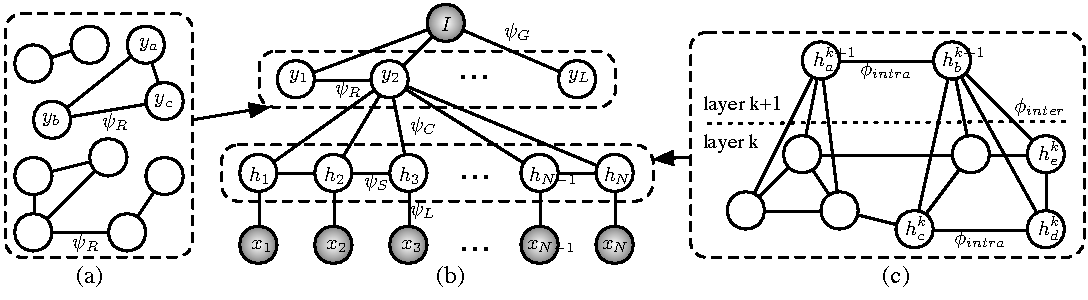
\includegraphics[width=0.95\linewidth]{graphmodel.pdf}
    \end{center}
    \caption{Example of a short caption, which should be centered.}
    \label{fig:graphmodel}
\end{figure*}

\subsection{Label Consistency}
We require that the superpixel labels be consistent with the image labels: if any superpixel $x_p$ takes the label $i$, then image label indicator $y_i=1$; otherwise $y_i=0$. Such constraints can be encode by the following potential:
\begin{equation}
    \psi_{C}(\boldsymbol{y},\boldsymbol{h}) = 
    C \cdot \sum_{i,p} I(y_i=0 \mbox{ and } h_p=i) 
\end{equation}
where $I(\cdot)$ is the indicator function and $C$ is a positive constant that penalizes any inconsistency between the global and local labels.

\subsection{Appearance Model and Topic Model}

We include both appearance and topic model as follow:
\begin{equation}
    \begin{aligned}
        \psi_{at}(h_p,x_p) = &- \log \big\{ w_1\phi_a(h_p,a_p,\theta_a) \\
        &+ w_2\phi_t(h_p,t_p,\theta_t) \big\} 
    \end{aligned}
\end{equation}
where $a_p, t_p$ are the appearance and topic feature vectors extracted from the superpixels, $\theta_a, \theta_t$ donate the parameters with repect to appearance model and topic model, $\{w_i\}|_{i=1}^2$ are the weighting coefficients for the unary terms. We define the appearance model $\phi_a(h_p,a_p,\theta_a) = f_{h_p}(a_p,\theta_a)$ and topic model $\phi_t(h_p,t_p,\theta_t) = g_{h_p}(t_p,\theta_t)$ measuring how well the local appearance $a_p$ and topic $t_p$ matches the semantic label $h_p$.

\subsection{Spatial Constraints and Hierarchical model}
We 
\begin{equation}
    \psi_{S}(h_p,h_q) =
    \begin{cases}
        \phi_{inter}(h_p,h_q) &\mbox{ if } | l_p - l_q | = 1,
        \\
        \phi_{intra}(h_p,h_q) &\mbox{ if } l_p = l_q,
        \\
        0 &\mbox{ otherwise }
    \end{cases}
\end{equation}
where $l_p$ indicates the quantization level that the superpixel $x_p$ belongs to. 
The inter-level energy cost $\phi_{inter}$ is defined as:
\begin{equation}
    \phi_{inter}(h_p,h_q) = \gamma \cdot O(x_p,x_q) \cdot I(h_p \neq h_q)
\end{equation}
where $O(x_p,x_q)$ refers to the intersection (overlapping area) of two superpixels, $I(\cdot)$ is the indicator function and $\gamma$ is the weighting coefficient. This formulation is based on the higher order constraints \cite{kohli2009robust,ladicky2009associative} that superpixels lying within the same clique are more likely to take the same label.
And the intra-level energy cost $\phi_{intra}$ is defined as:
\begin{equation}
    \phi_{intra}(h_p,h_q) = Sim(x_p,x_q) \cdot (1-R(h_p,h_q))
\end{equation}
where $Sim(x_p,x_q) \in [0,1]$ measures the visual similarity between superpixel $x_p$ and $x_q$, $R(h_p,h_q) \in [0,1]$ is a learnt correlation between label $h_p$ and $h_q$. Hence, we pay a high cost for the similar superpixels if they were assigned different labels and for the superpixels which were assigned an irrelevant label to the context.

\subsection{Label Correlation and Co-occurrence}


\subsection{Joint Inference with Alternate Procedure}
The energy minimization problem \eqref{eq:energyfunction} can be solved in the following two alternate optimization steps:
\begin{equation}
    \label{eq:binaryCRF}
    \begin{aligned}
        \boldsymbol{y}^* = \arg\min_{\boldsymbol{y}} &\sum_{i} {\psi_{G}(y_i,I)} + \frac{1}{2} \psi_{C}(\boldsymbol{y},\boldsymbol{h}^*) \\ &+ \sum_{1 \le i,j \le L} {\psi_{R}(y_i,y_j)}, 
    \end{aligned}
\end{equation}
\begin{equation}
    \label{eq:multiclassCRF}
    \begin{aligned}
        \boldsymbol{h}^* = \arg\min_{\boldsymbol{h}} &\sum_{p} {\psi_{at}(h_p,x_p)} + \frac{1}{2} \psi_{C}(\boldsymbol{y}^*,\boldsymbol{h}) \\ &+ \sum_{(p,q) \in \mathcal{E}}{\psi_{S}(h_p,h_q)}.
    \end{aligned}
\end{equation}
As a standard binary CRF problem, the first subproblem in Eq. \eqref{eq:binaryCRF} has an explicit solution which utilizes min-cut/max-flow algorithms (\eg the Dinic algorithm \cite{dinits1970algorithm}) to obtain the global optimal label configuration. And the second subproblem in Eq. \eqref{eq:multiclassCRF} reduces to an energy minimization for a multiclass CRF. Although finding the global optimum for this energy function has been proved to be a NP-hard problem, there are various approximate methods for fast inference, such as approximate \textit{maximum a posteriori} (MAP) methods (\eg graph-cuts \cite{boykov2001fast}). In this paper, we adopt \textit{move making} approach \cite{boykov2001fast} that finds the optimal $\alpha$-expansion \cite{boykov2001fast,kolmogorov2004energy} by converting the problems into binary labeling  problems which can be solved efficiently using graph cuts techniques. The energy obtain by $\alpha$-expansion has been proved to be within a known factor of the global optimum \cite{boykov2001fast}. Considering the two alternate optimization steps together, we summarize our XXXX in Algorithm \ref{alg:energy}.


\begin{algorithm}[htb]
    \caption{ Energy minimization }
    \label{alg:energy}
    \begin{algorithmic}[1]
        \State 123
    \end{algorithmic}
\end{algorithm}



\section{Appearance and Topic Model Generation}
\label{sec:appearancetopic}
We use Convolutional Neural Network (CNN) to encode the superpixels' appearance. CNN has made a significant breakthrough in object detection and semantic segmentation tasks \cite{girshick2013rich}. As demonstrated in \cite{girshick2013rich}, the classification network trained on ImageNet \cite{deng2009imagenet} can generalize well to the detection task. We train a classification model on ILSVRC with the same setup to \cite{girshick2013rich}, which uses five convolutional layers and three fully-connected layers. We represent each superpixel by the \textit{fc6} layer, which is the first fully-connected layer containing 4096 neurons. Therefore, the appearance representation of each superpixel is a feature vector with 4096 dimentions.

Moreover, we learn the latent category (known as topic model) from the superpixels. 



